\task{ В теплоизолированном цилиндре на расстоянии $L_1=80$ см друг от
  друга находятся два легкоподвижных теплопроводящих поршня.
  Пространство между ними заполнено водой, а снаружи на поршни
  действует атмосферное давление. Слева от левого поршня включили
  холодильник, который поддерживает постоянную температуру
  $t_1=-40^{\circ}$C, а справа от правого нагреватель, поддерживающий
  постоянную температуру $t_2=16^{\circ}$C. Через некоторое вре мя
  система пришла в стационарное состояние и расстояние между поршнями
  стало $L_2$. После этого поршни снаружи теплоизолировали и дождались
  установления теплового равновесия в цилиндре. Расстояние между
  поршнями стало $L_3$. Найдите $L_2$ и $L_3$. Плотность льда
  $\rho_{\mbox{\footnotesize{л}}} =900\mbox{ кг/м}^3$, плотность воды
  $\rho_{\mbox{\footnotesize{в}}} =1000\mbox{ кг/м}^3$, удельная
  теплоёмкость воды $c_{\mbox{\footnotesize{в}}} =4200\mbox{
    Дж/(кг}\cdot{}^{\circ}\mbox{C)}$, удельная теплоёмкость льда
  $c_{\mbox{\footnotesize{л}}} =2100 \mbox{Дж/(кг}
  \cdot{}^{\circ}\mbox{C)}$, удельная теплота плавления льда
  $\lambda=330$ кДж/кг, коэффициент теплопроводности льда в 4 раза
  больше коэициента теплопроводности воды.\\ \textit{Указание.}
  Считайте, что мощность теплового потока $P$ вдоль цилиндра, между
  торцами которого поддерживается постоянная разность температур
  $\Delta t$, равна: $$ P=\frac{kS\Delta t}{L}, $$ где
  $k$~---~коэффициент теплопроводности среды, $S$~---~площадь торца
  цилиндра, $L$~---~длина цилиндра. }

\begin{center}
  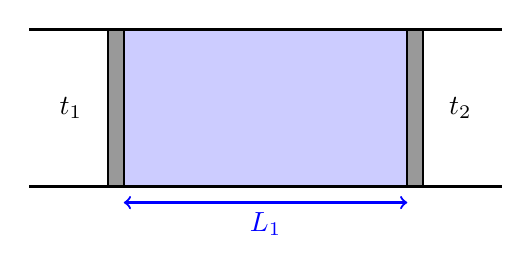
\begin{tikzpicture}
    \draw[fill=blue!20,thick] (1.2,0) rectangle (4.8,2);
    \draw[fill=gray!80,thick] (1,0) rectangle (1.2,2)
    node[midway,left=0.3cm] {$t_1$};
    \draw[fill=gray!80,thick] (4.8,0) rectangle (5,2)
    node[midway,right=0.3cm] {$t_2$};
    \draw[very thick] (0,2) -- (6,2);
    \draw[very thick] (0,0) -- (6,0);
    \draw[blue,thick,<->] (1.2,-0.2) -- (4.8,-0.2) node[midway, below]
    {$L_1$};
  \end{tikzpicture}
\end{center}
% Россия-2013, 9 класс